\chapter{\IfLanguageName{dutch}{Stand van zaken}{State of the art}}
\label{ch:stand-van-zaken}
% Tip: Begin elk hoofdstuk met een paragraaf inleiding die beschrijft hoe
% dit hoofdstuk past binnen het geheel van de bachelorproef. Geef in het
% bijzonder aan wat de link is met het vorige en volgende hoofdstuk.

% Pas na deze inleidende paragraaf komt de eerste sectiehoofding.

%Dit hoofdstuk bevat je literatuurstudie. De inhoud gaat verder op de inleiding, maar zal het onderwerp van de bachelorproef *diepgaand* uitspitten. De bedoeling is dat de lezer na lezing van dit hoofdstuk helemaal op de hoogte is van de huidige stand van zaken (state-of-the-art) in het onderzoeksdomein. Iemand die niet vertrouwd is met het onderwerp, weet nu voldoende om de rest van het verhaal te kunnen volgen, zonder dat die er nog andere informatie moet over opzoeken \autocite{Pollefliet2011}.

%Je verwijst bij elke bewering die je doet, vakterm die je introduceert, enz. naar je bronnen. In \LaTeX{} kan dat met het commando \texttt{$\backslash${textcite\{\}}} of \texttt{$\backslash${autocite\{\}}}. Als argument van het commando geef je de ``sleutel'' van een ``record'' in een bibliografische databank in het Bib\LaTeX{}-formaat (een tekstbestand). Als je expliciet naar de auteur verwijst in de zin, gebruik je \texttt{$\backslash${}textcite\{\}}.
%Soms wil je de auteur niet expliciet vernoemen, dan gebruik je \texttt{$\backslash${}autocite\{\}}. In de volgende paragraaf een voorbeeld van elk.

%\textcite{Knuth1998} schreef een van de standaardwerken over sorteer- en zoekalgoritmen. Experten zijn het erover eens dat cloud computing een interessante opportuniteit vormen, zowel voor gebruikers als voor dienstverleners op vlak van informatietechnologie~\autocite{Creeger2009}.
\section{\IfLanguageName{dutch}{Probleemstelling}{Problem Statement}}
\label{sec:probleemstelling}


\section{Definitie KMO}

Bedrijven kunnen opgedeeld worden volgens grootte. Er zijn drie groottes waarin er een onderscheid gemaakt wordt:

\begin{itemize}
    \item Kleine onderneming (KO)
    \item Middelgrote onderneming (MO)
    \item Grote onderneming (GO)
\end{itemize}

Volgens \textcite{Vlaio2014} is een ko of kleine onderneming een zelfstandig bedrijf met minder dan 50 werknemers én met een maximum jaaromzet van €10 miljoen of een maximum balanstotaal van €10 miljoen.

Een kmo of kleine of middelgrote onderneming is een zelfstandig bedrijf met minder dan 250 werknemers én met een maximum jaaromzet van €50 miljoen of een maximum balanstotaal van €43 miljoen.

Ondernemingen die ontdekken dat de drempel in het voorbij boekjaar overschreden is, verliezen pas de status van KMO (of ko) als deze situatie zich gedurende twee opeenvolgende boekjaren voordoet.

\newpage
Een onderneming moet voldoen aan elk van de drie voorwaarden om tot een bepaalde groottecategorie te behoren:

\begin{table}[ht]
    \centering
    \caption{Definitie KO, MO en GO}
    \begin{tabular}[t]{l>{\raggedright}p{0.2\linewidth}>{\raggedright\arraybackslash}p{0.3\linewidth}>{\raggedright\arraybackslash}p{0.18\linewidth}}
        \toprule
        \textbf{Groottecategorie} & \textbf{aantal werknemers \footnote{ Het aantal werknemers die bij de RSZ-ingeschreven zijn als VTE (voltijds equivalent)} } & \textbf{jaaromzet of jaarlijks balanstotaal} & \textbf{zelfstandigheid} \\
        \midrule
        KO & minder dan 50 & tot 10 miljoen of tot 10 miljoen & ja \\
        MO  &minder dan 250 & tot 50 miljoen of tot 43 miljoen & ja \\
        GO & vanaf 250 & meer dan 50 miljoen en meer dan 43 miljoen & ja \\
        \bottomrule
    \end{tabular}
\end{table}

%Afbeelding te plaatsen

Deeltijdwerknemers of werknemers die een jaar niet voor een bedrijf hebben gewerkt, worden proportioneel omgerekend naar "voltijdse werknemers" (bijvoorbeeld: twee deeltijdse werknemers zijn één voltijdse werknemer). Uitzendkrachten worden niet meegeteld.

Wanneer een onderneming een kmo-portefeuille aanvraagt, wordt op basis van deze criteria de grootte van de onderneming voorgesteld. De kmo-portefeuille verkrijgt deze gegevens via de Nationale Bank van België. De grootte van de onderneming wordt vastgesteld bij de eerste succesvolle steunaanvraag in een kalenderjaar en geldt voor de rest van het kalenderjaar.

De kmo-portefeuille controleert enkel de gegevens die gekoppeld zijn aan het ondernemingsnummer van de onderneming die de steun aanvraagt. Indien deze onderneming deel uitmaakt van een groep ondernemingen, moeten ook de criteria van andere ondernemingen (deelnemende ondernemingen en/of deelnemende ondernemingen) worden meegerekend volgens de definitie van KMO's in Europa.

\section{Verschil tussen staging en deployment}

In de IT-wereld heeft het woord staging een meerduidige betekenis. Een staging omgeving wordt zo beschreven als: ‘een kopie van de productieomgeving op een private server, dat dienst doet als veilige omgeving waarop wijzigingen kunnen worden getest’, zoals omschreven in \textcite(commonplaces2021). In tegenstelling tot deze definitie verwijst de term staging die in de context van deze bachelorproef wordt gebruikt naar de definitie die in de handleiding van \textcite(Vodafone2014) te vinden is: "Staging bereidt een toestel voor op enrollment."

Staging verwijst dus naar de basisconfiguratie die op alle toestellen op dezelfde manier wordt uitgevoerd om het toestel in kwestie operationeel te krijgen. Deze vaste installaties kunnen geautomatiseerd worden. In dat geval wordt het een taak genoemd. Deze taken (of tasks) verschillen sterk van bedrijf tot bedrijf, aangezien de behoeften van ene het bedrijf niet noodzakelijk dezelfde zijn als van het ander bedrijf. Er zijn echter veel taken die elk bedrijf moet uitvoeren. Er moet altijd een besturingssysteem of OS geïnstalleerd worden en de vereiste licenties moeten toegewezen worden. Daarnaast moet het apparaat lid worden van het bedrijfsdomein, de vereiste updates voor Windows moeten gedownload en geïnstalleerd worden, en de vereiste software moet aan het apparaat toegevoegd worden.

Volgens \textcite(techopedia2018) betekent deployment, wanneer gebruikt in de context van netwerkbeheer: "Deployment verwijst naar het proces dat doorlopen moet worden om een nieuwe computer of een nieuw systeem zo op te zetten, dat het klaar is om gebruikt te worden in de werkomgeving". Deployment is dus een zeer breed concept. Het beschrijft het gehele proces dat moet worden doorlopen voordat een systeem effectief kan gebruikt worden. Dit omsluit alle installaties, configuraties, specifieke wijzigingen en tests die moeten worden uitgevoerd voordat het systeem volledig operationeel is.

\section{Noodzakelijkheid van deployment tools}

Deployment tools worden in vele bedrijven gebruikt om te voorkomen dat beheerders niet elk apart toestel in een netwerk manueel moeten opzetten. Op deze manier kan men te allen tijde een duidelijk beeld verkrijgen over de staat waarin de toestellen zich binnen het netwerk bevinden. Via deze tools kan veel tijd bespaard worden en wordt de kans op fouten, die gepaard gaan met het manueel opzetten van toestellen, verkleind. \autocite{Goessens2020}


\section{Werking van deployment tools}

De werking van deployment tools verschilt van tool tot tool. Er zijn tools die gebruik maken van imaging en er zijn tools die een van een bestaande image vertrekken en applicaties, policies, certificaten, etc. pushen zoals bij Microsoft Intune het geval is. Elke tool heeft ook een verschillende set van functionaliteiten. Als een apparaat tot een operationeel niveau moet gebracht worden, dan moeten er verschillende stappen overlopen worden. Er moet uiteraard een OS of Operating System geïnstalleerd worden, het apparaat moet het domein van het bedrijf joinen en er moeten policies, applicaties, certificaten, etc. gepusht worden. \autocite{Goessens2020}

MDT maakt hiervoor gebruik van een task sequence. Nadat deze task sequence is aangemaakt kan de PXE boot\footnote{Preboot execution environment is een reeks normen die een computer in staat stelt een besturingssysteem (OS) te laden via een netwerkverbinding.} van het nieuwe systeem worden uitgevoerd. Hiervoor is een centraal punt nodig dat het nieuwe apparaat kan aanspreken. Bij MDT wordt dit een sharepoint genoemd, meer bepaald een deployment share. \autocite{Goessens2020}

In het geval van Intune Autopilot gebeurt dit via een Intune Tenant die onder meer verschillende applicaties en configuration profiles bevat die over een internet connectie gepusht worden naar het nieuwe apparaat bij de eerste opstart ervan. Het apparaat moet ook geregistreerd en voorbereid worden voor mobile management.

\section{Overzicht van de verschillende beschikbare tools voor laptop deployment binnen een Windows bedrijfsomgeving}

In deze sectie van de literatuurstudie wordt er een overzicht gegeven van een paar beschikbare tools voor laptop deployment binnen een Windows bedrijfsomgeving. De opbouw van deze sectie ziet er als volgt uit:

\begin{itemize}

    \item Windows installeren

    \item Installeren van applicaties

    \item Installeren van policies

\end{itemize}

Bij elke stap van het deployment proces wordt besproken hoe dit in zijn werk gaat voor de volgende drie tools:

\begin{itemize}

    \item WinPE\footnote{Windows PE (WinPE) is een klein besturingssysteem dat wordt gebruikt om Windows desktop edities, Windows Server, en andere Windows besturingssystemen te installeren, te implementeren en te repareren.} via USB

    \item WDS/MDT

    \item Microsoft Intune: Windows Autopilot

\end{itemize}


Bij elke deploment tool worden ook de bijhorende struikelblokken aangekaart. De volgorde van deze deployment tools loopt parallel met de chronologie waarin de technieken doorheen de jaren zijn toegepast. Vroeger moesten IT-werknemers laptop deployment manueel uitvoeren via een USB-stick. Via deze USB-stick werd dan WinPE uitgevoerd. Vervolgens wordt uitgelegd hoe IT-werknemers via WDS/MDT laptop deployment volledig kunnen automatiseren. Ten slotte wordt een van de nieuwste vormen van laptop deployment omschreven die niet meer zoals WDS/MDT afhankelijk is van on-premise resources, maar volledig in de cloud werkt: Microsoft Intune Windows Autopilot.

\subsection{Windows installeren}

Een besturingssysteem is een interface tussen de gebruiker van een computer en de hardware van een computer. Een besturingssyteem, in dit geval Windows OS, is de software die alle basistaken afhandelt, zoals bestandsbeheer, geheugenbeheer, procesbeheer en I/O\footnote{Input/Output of invoer/uitvoer}, en randapparatuur zoals drives en printers aanstuurt. Er zijn veel verscheidene besturingssystemen op de markt aanwezig zoals Windows OS, Linux OS, MacOS, etc.\autocite{tutorialspoint2022} In dit onderzoek wordt enkel rekening gehouden met het eerste vernoemde besturingssysteem, namelijk Windows OS. Bij laptop deployment is de installatie van een Windows-besturingssyteem uiteraard een belangrijke stap in het proces.

Er zijn veel gevallen waarin een besturingssysteem opnieuw moet geïnstalleerd worden. Windows wordt bijvoorbeeld opnieuw geïnstalleerd  als er een ernstige fout optreedt, als de harde schijf beschadigd is, of als het systeem moet upgraden/downgraden. How to Install Windows 10, 8.1 or 7 Using a Bootable USB.\autocite{softwarekeep2022}

\textbf{WinPE via USB}

Omdat cd's en dvd's steeds minder praktisch zijn, worden veel computers en laptops niet meer geleverd met een station om fysieke schijven te lezen en te schrijven. Deze fysieke schijven worden als installatiemedium gebruikt om over de nodige installatiebestanden te beschikken voor de installatie van een besturingssysteem. Een andere optie om een Windows-besturingssysteem te installeren is via een opstartbare USB-stick. Hoewel dit op het eerste gezicht misschien onpraktisch klinkt, hebben USB-sticks een enorm voordeel ten opzichte van schijven. USB's zijn heel toegankelijk, gezien het feit dat bijna elke computer een USB-poort heeft om externe apparaten op aan te sluiten. Het is de gemakkelijkste en meest gestroomlijnde methode om een besturingssysteem te installeren. Tegenwoordig kan er een opstartbare USB-stick gemaakt worden om verschillende versies van Windows te installeren op eindgebruiker apparaten.\autocite{softwarekeep2022}

De werkwijze via een USB-stick begint met het formatteren van de schijf en de primaire partitie in te stellen als actief.

Nadien wordt het FAT32-bestandssysteem\footnote{FAT32 is een bestandssysteem voor opslagmedia (zoals harde schijven, USB-sticks en solid state drives) met een 32 bits-File Allocation Table.} geselecteerd om zowel BIOS\footnote{Het BIOS (Basic Input / Output System) is een programma dat door de microprocessor van een computer wordt gebruikt om het computersysteem op te starten nadat het is ingeschakeld.}-gebaseerde als UEFI\footnote{Unified Extensible Firmware Interface is bedoeld om na verloop van tijd BIOS te vervangen.}-gebaseerde PC's te kunnen booten. De Windows USB installatiedrive is geformatteerd als FAT32 met een limiet van 4GB bestandsgrootte. Als de afbeelding groter is dan de maximale bestandsgrootte (4 gigabyte) moet de Windows image opgedeeld worden in kleinere bestanden.\autocite{EliotSeattle2021}

Vervolgens wordt de Windows setup gekopieerd naar de USB-stick zodat deze kan worden aangesloten op een nieuwe computer om Windows te installeren. Zodra de USB-stick is aangesloten op de nieuwe machine, kan deze machine worden opgestart. Tijdens de opstart wordt het boot device\footnote{Een boot device is elk stukje hardware dat de bestanden bevat die nodig zijn om een computer te laten opstarten.} keuzemenu voor de computer geopend door op de Esc-, F10- of F12-toets te drukken (dit is afhankelijk van het model van de computer). In dit venster wordt voor de optie gekozen om de PC op te starten vanaf de USB-stick. De Windows setup wordt opgestart en de instructies van deze setup worden verder uitgevoerd.\autocite{EliotSeattle2021}

\textbf{Struikelblokken}

Laptop deployment via een USB-stick brengt veel struikelblokken met zich mee. Allereerst is dit een methode die enorm veel tijd in beslag neemt voor de IT-werknemer. Via een USB-stick moet de IT-werknemer alle laptops binnen de bedrijfsomgeving manueel opstarten en de Windows setup doorlopen. Er is dus geen sprake van automatisatie in het deployment proces om tijd te besparen.

Vervolgens moet de IT-werknemer de Windows image op de USB-stick up-to-date houden. Ook dit neemt veel tijd en energie in beslag. Deze methode is dus niet geschikt om in een KMO te gebruiken voor laptop deployment, waar vaak tientallen of honderden werknemers in het bedrijf aanwezig zijn.

Volgens \textcite{tedhudek2021} maakt de standaardinstallatie van Windows PE  gebruik van het FAT32-bestandsformaat, dat zijn eigen beperkingen heeft, waaronder een maximale bestandsgrootte van 4 GB en een maximale schijfgrootte van 32 GB.

Vervolgens ondersteunt Windows PE volgens \textcite{tedhudek2021} geen van de volgende functies:

\begin{itemize}

    \item Gebruik van een bestandsserver of een Terminal Server.

    \item Deel worden van een netwerkdomein.

    \item Verbinding maken met een IPv4 netwerk vanuit Windows PE via een IPv6 netwerk.

    \item Kantoor op afstand. (telewerk)

    \item .MSI installatiebestanden.

    \item Starten vanaf een pad dat niet-Engelse tekens bevat.

    \item 64-bits toepassingen uitvoeren op 32-bits versies van Windows PE.

    \item Gebundelde apk's\footnote{Android Package} toegevoegd via DISM\footnote{Microsoft Windows Deployment Image Servicing and Management (DISM) is een softwareprogramma dat IT-beheerders kunnen gebruiken via  PowerShell om een Windows-desktopimage of harde schijf te mounten en te onderhouden voordat deze aan gebruikers wordt aangeboden.} (.appxbundle pakketten).

\end{itemize}

\textbf{MDT/WDS}

De Microsoft Deployment Toolkit (MDT, voorheen bekend als Business Desktop Deployment) is een gratis tool voor het automatiseren van de implementatie van Windows- en Windows Server-besturingssystemen die gebruik maken van de Windows Assessment and Deployment Kit (ADK) voor Windows 10. MDT is een geïntegreerde verzameling tools, processen en richtlijnen voor het automatiseren van desktop- en serverimplementaties. Een IT-werknemer kan het gebruiken om een referentie-image te maken of het gebruiken als een volledige implementatieoplossing.\autocite{Christian2021}

MDT werkt met WDS samen door een PXE-serverfunctionaliteit over het netwerk te leveren en vooraf gegenereerde MDT-opstartbestanden te gebruiken om verbindingen met MDT-shares op te zetten. Als de client WDS-besturingssysteemimages gebruikt, moet de IT-werknemer deze bootimages in WDS importeren. Met WDS kan een IT medewerker ook images van referentieapparaten vastleggen en PXE gebruiken om die images te implementeren op verschillende apparaten in de bedrijfsomgeving met ondersteuning van stuurprogramma's. MDT is een meer ontwerpgericht hulpprogramma, maar MDT maakt boot images\footnote{Een boot image is een soort schijfimage (een computerbestand dat de volledige inhoud en structuur van een opslagmedium bevat)} in verschillende stapsgewijze implementatievolgorden.\autocite{Christian2021}

WDS (Windows Deployment Services) is een servertechnologie van Microsoft voor het uitvoeren van netwerkgebaseerde installaties van Windows-besturingssystemen (OS). WDS is een gewijzigde versie van de Remote Installation Service (RIS) en maakt de implementatie van het Windows-besturingssysteem mogelijk. Een IT-werknemer kan WDS gebruiken om nieuwe clients te configureren via netwerkgebaseerde instellingen.\autocite{Christian2021}

\textbf{Struikelblokken}

MDT is een gratis tool van Microsoft, maar het kost veel tijd om de omgeving op te zetten en het bedrijf is afhankelijk van on-premise resources. Volgens \textcite{Dunford2022} spenderen IT professionals weken of zelfs maanden om MDT op te zetten in de bedrijfsomgeving en deze uit te testen. Bovendien verspilt de IT-werknemer veel tijd die nodig is om een apparaat daadwerkelijk te deployen. Dit is kostbare tijd die de IT medewerker weghoudt van andere belangrijke initiatieven en projecten.



\textbf{Microsoft Intune: Windows Autopilot}

Volgens \textcite{LanceHarmstrong2021} behoort het installeren van Windows niet tot de taken die Windows Autopilot uitvoert. Autopilot is geen imaging. Intune doet niet aan imaging. Autopilot is provisioning. Het werkt verder op de lokale image van de computer afkomstig van de fabrikant. Het typische scenario is dat de machines van de OEM imaged toekomen in het bedrijf, en de OEM gebruikt de eigen provider tenant om de UUID (Universally Unique Identifier) van het apparaat aan de Intune tenant van het bedrijf te koppelen.

Autopilot is slechts een geautomatiseerde methode voor het implementeren van applicaties, bedrijfspolicies en configuraties op een machine die rechtstreeks van de OEM wordt geïmaged. In wezen wordt imaging overgeslagen, ofwel omdat er niet echt een image nodig is, of omdat de OEM betaald wordt om het voor het bedrijf te doen.



\textbf{Struikelblokken}

Windows Autopilot installeert technisch gezien geen OS met een voorgedefinieerd OS image zoals WDS/MDT dat doet. Het gebruikt eigenlijk de lokale image op het apparaat en configureert het out-of-the-box. Windows Autopilot is dus een NextGen vervanging van WDS/MDT, maar alleen voor Windows 10 of 11 installaties. Als een IT-werknemer een aangepaste image wilt gebruiken, moet WDS/MDT gebruikt worden zoals voorheen (of een ander alternatief van derden).



\subsection{Installeren van applicaties}



\textbf{WinPE via USB}

Het doorvoeren van bedrijfspolicies via WinPE gebeurt door scripts die op de image van de USB-stick worden uitgevoerd. Deze scripts kunnen dus enkel bij eerste opzet van een apparaat worden uitgevoerd.



\textbf{Struikelblokken}

Wanneer een IT-werknemer een applicatie wil installeren of updaten op een apparaat moet dit manueel gebeuren op de doelcomputer of via een script op de doelcomputer. Er is dus geen mogelijkheid om dit op afstand te doen. De IT-werknemer moet ook manueel de wizard van de installatie doorlopen. Als de IT-werknemer dit voor elk apparaat in een bedrijf van honderden werknemers moet doen, dan neemt dit heel veel tijd in beslag tegenover geautomatiseerde deployment tools.



\textbf{MDT/WDS}

Volgens \textcite{RDRIT2022} bestaan er twee methoden om applicaties via MDT te installeren. Een eerste methode is om een applicatie te installeren via de Windows Deployment Wizard. Een tweede methode werkt met een task sequence in de MDT Workbench.

Voorafgaand moet de applicatie toegevoegd worden in de MDT console (of de MDT Workbench). Dit is noodzakelijk voor beide methodes die in de vorige alinea geïntroduceerd werden. Hiervoor moet de IT-werknemer een aparte wizard\footnote{handleiding bij installatie} volgen die bepaalde acties vereist zoals het meegeven van de bronmap, de naam van de doelmap van de applicatie en een commando voor de stille installatie. Het doorlopen van deze wizard resulteert in map die gecreëerd wordt in de deployment share / Application folder.

De eerste methode omvat de installatie van een applicatie via de Windows Deployment Wizard. Als de applicatie beschikbaar is in MDT, verschijnt er tijdens het deployment proces een extra venster waarin deze beschikbaar zijn voor installatie. In dit venster worden de nodige applicaties aangevinkt om te installeren.

%De afbeelding hieronder verwijst naar dit venster. https://static.rdr-it.com/images/rdr-img-message.png

%\begin{figure}
%    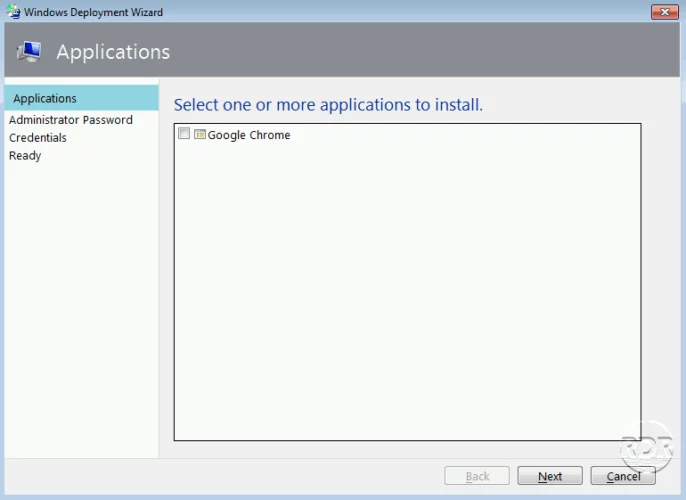
\includegraphics[width=\linewidth]{Appwizard}
%    \caption{Windows Deployment Wizard}
%    \label{fig:figuur1}
%\end{figure}

De tweede methode werkt via een task sequence. Het is mogelijk om vanuit de OS installation sequence applicaties geforceerd te deployen. Dit gebeurt via de Custom Tasks in de task sequence eigenschappen.

%afbeelding erbij plaatsen https://static.rdr-it.com/images/rdr-img-message.png

\textbf{Struikelblokken}

Er is een directe connectie nodig van de doelcomputer naar de WDS server. De WDS server haalt de images op vanuit de deployment share van MDT met de bijhorende applicaties of task sequence. Dit zorgt ervoor dat dit niet op afstand kan gebeuren. Als een on-premise resource (Domein Controller, Server met WDS en MDT, etc.) uitvalt, dan kan de IT-werknemer geen images meer deployen op een doelcomputer.


\textbf{Microsoft Intune: Windows Autopilot}

In de Endpoint Manager van Microsoft Intune kan een IT-werknemer applicatie-profielen opstellen om applicaties te installeren op computers van eindgebruikers. Er zijn veel mogelijkheden om apps via Intune naar eindgebruikers te pushen: Microsoft store apps, Managed Google Play apps, Windows apps (Win32), Microsoft 365 apps voor Windows 10, Business Line Apps, etc. Een applicatie wordt op device- of op user-niveau geïnstalleerd. Applicaties die op device niveau geïnstalleerd worden, beginnen direct met installeren zodra de computer verbinding maakt met het internet en met de Intune tenant\footnote{Een tenant is een specifieke instantie van Azure Active Directory (Azure AD) waar uw abonnement op Intune wordt gehost} van de organisatie. Hiervoor moet de werknemer eerst inloggen via een Microsoft-account.
\autocite{Erikre2022}

bf{Struikelblokken}

Er is nog altijd ruimte voor fouten bij installaties via Intune. De internetverbinding kan bijvoorbeeld wegvallen, waardoor de installatie onderbroken wordt. Dan hangt een succesvolle installatie af van de applicatiewizard die wel of niet correct sluit en opnieuw zal doorlopen worden op de achtergrond. In de cloud opslag staat er een limiet ingesteld op de maximale grootte van een file die geüpload wordt (8 gigabyte).\autocite{Erikre2022}



\subsection{Installeren van policies}



\textbf{WinPE via USB}

Het doorvoeren van bedrijfspolicies via WinPE gebeurt door scripts die op de image van de USB-stick worden uitgevoerd. Deze scripts kunnen dus enkel bij eerste opzet van een apparaat worden uitgevoerd. Wanneer een IT-werknemer een bedrijfpolicy wil updaten, dan moet dit manueel gebeuren op het apparaat van elke eindgebruiker.



\textbf{Struikelblokken}

Wanneer een IT-werknemer een bedrijfspolicy wil veranderen op een apparaat moet dit manueel gebeuren op de doelcomputer of via een script op de doelcomputer van de eindgebruiker. Er is dus geen mogelijkheid om dit op afstand te doen en dit zorgt voor ontzettend veel tijdverlies.

Het toetreden tot het netwerk domein van de organisatie is niet mogelijk via WinPE volgens \textcite{tedhudek2021}. Bedrijven met honderden werknemers vereisen een eigen en apart domein. WinPE ondersteunt geen toetreding tot het netwerk domein en dit vormt dus een groot probleem voor hedendaagse bedrijven. \autocite{EliotSeattle2021}



\textbf{MDT/WDS}

Om policies te installeren op een computer van een eindgebruiker via MDT moet de IT-werknemer een externe tool downloaden, nl. LGPO.exe. Deze tool wordt gekopieerd naar de deployment share waarna de task sequence in de MDT Workbench aangepast wordt om de policies lokaal te kopiëren en via de LGPO.exe te installeren.\autocite{Arwidmark2016}


\textbf{Struikelblokken}

Zoals vermeld bij de struikelblokken van het installeren van applicaties via WDS/MDT, is er ook voor het installeren van de policies een directe connectie nodig van de doelcomputer naar de WDS server. De doelcomputer moet binnen hetzelfde netwerk aanwezig zijn en dit kan dus niet op afstand uitgevoerd worden. Als een on-premise resource (Domein Controller, Server met WDS en MDT, etc.) uitvalt, dan kan de IT-werknemer geen images (waar deze policies opstaan) meer deployen op een doelcomputer.


\textbf{Microsoft Intune: Windows Autopilot}

Via Microsoft Intune worden policies gepushed naar werknemers via configuratieprofielen of configuration profiles. Deze configuration profiles worden toegewezen aan groepen binnen de Intune tenant. Deze groepen bestaan uit 2 soorten entiteiten: gebruikers of machines. Een mix van beide is niet mogelijk. Een groep kan dus enkel uit gebruikers of enkel uit machines bestaan om zo fouten te voorkomen bij installaties of updates.



\textbf{Struikelblokken}

Zoals vermeld in de struikelblokken van het installeren van applicaties via Intune, kan ook hier een internetconnectie die wegvalt voor problemen zorgen.


\section{Conclusie stand-van-zaken}

\textbf{WinPE via USB}

Deze methode is niet geschikt om in een KMO te gebruiken voor laptop deployment, waar vaak tientallen of honderden werknemers in het bedrijf aanwezig zijn. Het zorgt voor enorm veel tijdverlies en is niet flexibel genoeg om frequent nieuwe bedrijfspolicies of applicaties te installeren.

\textbf{MDT/WDS}

Deze methode is een goede oplossing voor KMO's met honderden werknemers. Alles kan geautomatiseerd worden, maar er is een directe connectie nodig naar de WDS server. Een computer deployen op afstand is dus geen mogelijkheid.

\textbf{Microsoft Intune: Windows Autopilot}

Microsoft Intune is een platform dat volledig in de cloud werkt en dus geen directe connectie vereist naar on-premise resources. Dit zorgt ervoor dat deze service gebruikt kan worden op afstand en op elk tijdstip.




